% Renewable Energy and Development, 2000-2024: technical report
% Compile with pdflatex + bibtex (Overleaf: upload this folder as a zip; it compiles as is).
\documentclass[11pt,a4paper]{article}

% ---------------------------------------------------------------- packages
\usepackage[a4paper,margin=2.5cm,headheight=14pt]{geometry}
\usepackage{mathpazo}
\usepackage[scaled=0.92]{helvet}
\usepackage[utf8]{inputenc}
\usepackage{microtype}
\usepackage{amsmath,amssymb}
\usepackage{graphicx}
\usepackage{booktabs,tabularx,multirow}
\usepackage{caption}
\usepackage{float,placeins}
\usepackage[dvipsnames,table]{xcolor}
\usepackage{enumitem}
\usepackage{titlesec}
\usepackage{fancyhdr}
\usepackage{tikz}
\usetikzlibrary{arrows.meta,positioning,fit,backgrounds}
\usepackage[most]{tcolorbox}
\usepackage[numbers,sort&compress]{natbib}
\usepackage{xurl}
\usepackage[colorlinks=true,linkcolor=accent,citecolor=accent,urlcolor=linkblue,
            pdftitle={Renewable Energy and Development, 2000-2024: Technical Report},
            pdfauthor={Sahil},pdfsubject={Energy transition data analysis}]{hyperref}
\usepackage{doi}

% ---------------------------------------------------------------- style
\definecolor{accent}{HTML}{1B8A6B}
\definecolor{linkblue}{HTML}{1D5AA6}
\definecolor{ink2}{HTML}{52514E}
\definecolor{boxbg}{HTML}{F1F7F4}

\captionsetup{font=small,labelfont={bf,sf},format=hang,margin=0.5em}
\setlist{itemsep=2pt,topsep=4pt}
\titleformat{\section}{\sffamily\Large\bfseries}{\color{accent}\thesection}{0.7em}{}
\titleformat{\subsection}{\sffamily\large\bfseries}{\color{accent}\thesubsection}{0.6em}{}
\titleformat{\subsubsection}{\sffamily\normalsize\bfseries}{}{0em}{}
\titlespacing*{\section}{0pt}{1.6em}{0.6em}
\titlespacing*{\subsection}{0pt}{1.2em}{0.4em}

\pagestyle{fancy}
\fancyhf{}
\renewcommand{\headrulewidth}{0.3pt}
\fancyhead[L]{\sffamily\small\color{ink2}Renewable Energy and Development, 2000--2024}
\fancyhead[R]{\sffamily\small\color{ink2}Technical report}
\fancyfoot[C]{\sffamily\small\thepage}

% "Why this choice" box
\newtcolorbox{why}[1][Why this choice]{enhanced,breakable,colback=boxbg,colframe=accent,
  boxrule=0pt,leftrule=2.5pt,arc=2pt,left=8pt,right=8pt,top=5pt,bottom=5pt,
  fonttitle=\sffamily\bfseries\small,coltitle=accent,attach title to upper={\ },title={#1.}}

\newcommand{\pp}{\,pp}
\newcommand{\code}[1]{\texttt{\small #1}}

% ================================================================= document
\begin{document}

% ---------------------------------------------------------------- title page
\begin{titlepage}
\setlength{\parindent}{0pt}
\vspace*{2.5cm}
{\sffamily\small\bfseries\color{accent} TECHNICAL REPORT \quad$\cdot$\quad VERSION 1.2 \quad$\cdot$\quad OCTOBER 2026\par}
\vspace{0.6cm}
{\sffamily\fontsize{28}{34}\selectfont\bfseries Renewable Energy and Development, 2000--2024\par}
\vspace{0.4cm}
{\Large\color{ink2} How the world's electricity mix is changing, how renewable energy relates to national income, and how this was measured\par}
\vspace{1.2cm}
{\large\sffamily\bfseries Sahil\par}
{\color{ink2} M.S.E.\ in Data Science, Johns Hopkins University\par}
\vspace{1.4cm}

\begin{tcolorbox}[enhanced,colback=boxbg,colframe=accent,boxrule=0pt,leftrule=3pt,arc=2pt,left=10pt,right=10pt,top=8pt,bottom=8pt]
\textbf{\sffamily Summary.} This report documents an end-to-end data project on the global energy transition. It combines World Bank and United Nations data on renewable energy for 215 countries (2000--2021) with Ember's electricity-generation data by source for 214 countries (2000--2024). It explains the motivation, every data source, every processing decision, every statistical method and the reason it was chosen, the results, and their limitations. The typical country's renewable share of electricity roughly doubled between 2000 and 2021, and worldwide renewables rose from 19\% to 32\% of electricity by 2024. ``Renewable share'' behaves very differently depending on whether it counts electricity or all energy use. Countries that started with low renewable shares are catching up, and national income explains little of the variation in clean electricity.
\end{tcolorbox}

\vspace{1cm}
{\small\begin{tabular}{@{}ll@{}}
\textbf{\sffamily Code and data} & \url{https://github.com/sahiljangra12/energy-transition-analysis} \\[2pt]
\textbf{\sffamily Interactive dashboard} & \url{https://sahiljangra12.github.io/energy-transition-analysis/} \\[2pt]
\textbf{\sffamily Licence} & Code: MIT. Data: original providers' terms (see Section~\ref{sec:data}).
\end{tabular}}
\vfill
{\small\color{ink2} Every number in this report is produced by the pipeline in the repository (\code{python -m energy\_transition}) and is checked by automated tests on every change.\par}
\end{titlepage}

\tableofcontents
\clearpage

% ================================================================= 1
\section{Motivation and research questions}\label{sec:motivation}

The United Nations' Sustainable Development Goal 7 asks countries to ``ensure access to affordable, reliable, sustainable and modern energy for all''. Its target 7.2 is to ``increase substantially the share of renewable energy in the global energy mix'' by 2030 \citep{un_2030}. Progress is tracked mainly through a single number, the renewable share of total final energy consumption (indicator 7.2.1), published every year by the custodian agencies in the \emph{Tracking SDG~7} report \citep{tracking_sdg7}.

A single headline number hides a lot. Three things motivated this project:

\begin{enumerate}
  \item \textbf{How we measure ``the trend'' matters.} The set of countries that report data changes from year to year. A simple median across whoever reports can rise or fall because of who joined, not because anything changed.
  \item \textbf{``Renewable'' means different things in different places.} In the poorest countries most energy is wood and charcoal burned for cooking, which official statistics count as renewable. A high renewable share there signals poverty, not a clean-energy transition. Electricity is a better lens on the modern transition, but even there a large share comes from hydropower built decades ago.
  \item \textbf{Income is often assumed to drive the transition.} Richer countries can afford new technology, but they also use more fossil energy. Whether income predicts renewable energy, and whether it does so within countries over time or only across countries, is an empirical question.
\end{enumerate}

The project therefore asks four questions:

\begin{description}[leftmargin=2.2em,style=sameline,font=\sffamily\bfseries\color{accent}]
  \item[Q1] How has the renewable share of electricity changed across countries since 2000, and does the answer depend on how the trend is measured?
  \item[Q2] How does renewable energy relate to national income, and does that depend on whether we count electricity or all energy use?
  \item[Q3] Which countries changed most between 2011 and 2021, and are countries with low renewable shares catching up?
  \item[Q4] Where does each country's electricity actually come from, source by source, and how has that mix changed up to 2024?
\end{description}

Questions Q1--Q3 are answered with statistics and regression models (Sections~\ref{sec:methods} and~\ref{sec:results}). Question Q4 is answered with an interactive country explorer (Section~\ref{sec:dashboard}), so that any reader can look up the country they care about.

% ================================================================= 2
\section{Data sources}\label{sec:data}

All data are public. Table~\ref{tab:sources} lists every source, and the subsections explain what each measures and why it was used.

\begin{table}[H]
\centering\small
\caption{Data sources used in the project.}\label{tab:sources}
\begin{tabularx}{\textwidth}{@{}p{3.1cm}Xp{2.7cm}p{1.9cm}@{}}
\toprule
\textbf{Source} & \textbf{Indicator} & \textbf{Coverage used} & \textbf{Used for} \\
\midrule
World Bank \citep{wb_elc_rnew} & \href{https://data.worldbank.org/indicator/EG.ELC.RNEW.ZS}{EG.ELC.RNEW.ZS}: renewable electricity output, \% of total electricity output & 2000--2021, 198--205 countries a year & Q1, Q2, Q3 \\
World Bank \citep{wb_fec_rnew} & \href{https://data.worldbank.org/indicator/EG.FEC.RNEW.ZS}{EG.FEC.RNEW.ZS}: renewable energy, \% of total final energy consumption & 2021 cross-section & Q2 \\
UN SDG database \citep{un_sdg_db,un_721_meta} & \href{https://unstats.un.org/sdgs/metadata/files/Metadata-07-02-01.pdf}{SDG 7.2.1}: renewable energy share in total final energy consumption & 2021 and 2023; 225 countries and areas & Q2 (cross-check) \\
World Bank \citep{wb_gdppc} & \href{https://data.worldbank.org/indicator/NY.GDP.PCAP.CD}{NY.GDP.PCAP.CD}: GDP per capita, current US\$ & 2000--2021 & Q2, Q3 \\
World Bank \citep{wb_pop} & \href{https://data.worldbank.org/indicator/SP.POP.TOTL}{SP.POP.TOTL}: total population & 2000--2021 & Weights and filters \\
Ember and Energy Institute, via Our World in Data \citep{ember,ei_review,owid_energy_repo} & \href{https://github.com/owid/energy-data}{Electricity generation by source}, TWh: coal, gas, oil, nuclear, hydro, wind, solar, bioenergy, other renewables & 2000--2024, 211--213 countries a year (196 in 2024) & Q4 \\
\bottomrule
\end{tabularx}
\end{table}

\subsection{World Bank World Development Indicators}
The World Bank publishes the renewable electricity and renewable final-energy series, GDP per capita and population through its Indicators API \citep{wb_api}. The responses were downloaded once and stored unchanged in the repository (Section~\ref{sec:processing}). The renewable electricity series ends in 2021 for most countries, which sets the end of the trend and regression analysis.

\begin{why}
The World Bank series are the most widely used cross-country source, they share one set of country codes, and they are available as a clean API. Using one provider for the outcome, income and population avoids mismatches between country lists.
\end{why}

\subsection{UN SDG indicator 7.2.1}
The UN Statistics Division's Global SDG Indicators Database \citep{un_sdg_db} publishes the official SDG 7.2.1 series. It measures the same concept as the World Bank's final-energy series and comes from overlapping underlying sources (IEA and UN energy statistics), but it covers more countries and areas (225 in 2023) and more recent years. It identifies countries by UN M49 numeric codes \citep{m49}.

\begin{why}
It is the official indicator for SDG target 7.2, so results stated in its terms connect directly to the policy debate. It also serves as a cross-check on the World Bank final-energy figures. The two are not independent confirmations of each other, a point repeated in the limitations.
\end{why}

\subsection{Electricity generation by source (Ember, via Our World in Data)}
The World Bank series gives only a renewable \emph{share}; it cannot separate hydropower from wind and solar, and it stops in 2021. For the country explorer, generation by source was taken from Our World in Data's energy dataset \citep{owid_energy,owid_energy_repo}, which compiles Ember's yearly electricity data \citep{ember} and the Energy Institute's Statistical Review of World Energy \citep{ei_review}. The file was downloaded on 15 October 2026 (SHA-256 of the uncompressed file begins \code{266f2e2baad79753}) and is stored unchanged. It is published under a CC BY 4.0 licence.

\begin{why}
Ember is the standard open source for electricity by fuel, it runs to 2024, and Our World in Data distributes it as a single versioned file on GitHub with consistent country codes. This makes it possible to show where each country's electricity comes from, and it addresses two weaknesses of the World Bank series (no breakdown by source and no data after 2021).
\end{why}

% ================================================================= 3
\section{Data processing}\label{sec:processing}

Figure~\ref{fig:pipeline} shows the pipeline. One command (\code{python -m energy\_transition}) rebuilds everything from the raw files.

\begin{figure}[H]
\centering
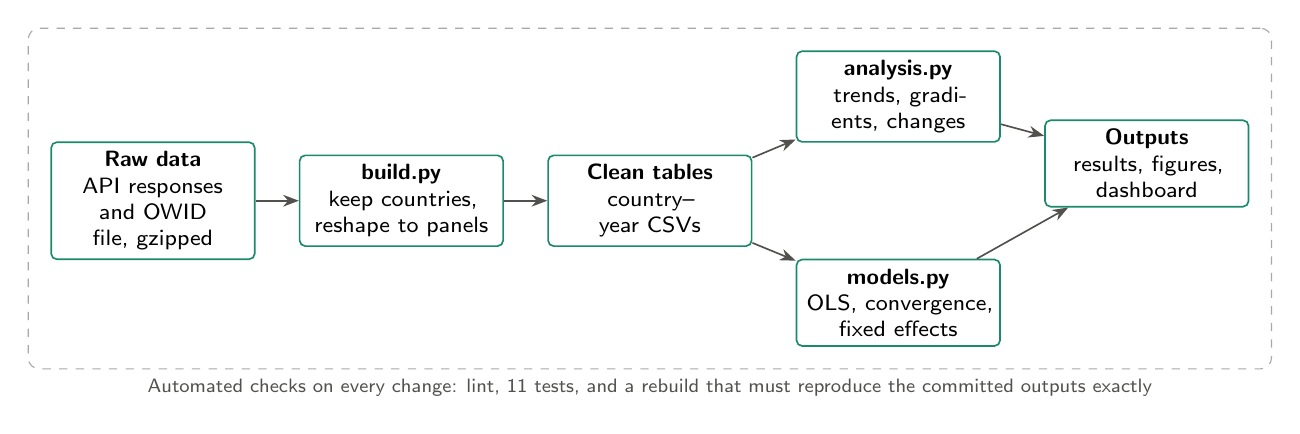
\begin{tikzpicture}[
  node distance=0.55cm and 0.55cm,
  box/.style={draw=accent,rounded corners=2pt,fill=white,align=center,font=\sffamily\footnotesize,minimum height=1.05cm,text width=2.35cm,line width=0.6pt},
  arr/.style={-{Stealth[length=2mm]},color=ink2,line width=0.6pt}]
\node[box] (raw) {\textbf{Raw data}\\API responses and OWID file, gzipped};
\node[box,right=of raw] (build) {\textbf{build.py}\\keep countries, reshape to panels};
\node[box,right=of build] (clean) {\textbf{Clean tables}\\country--year CSVs};
\node[box,above right=0.15cm and 0.55cm of clean] (an) {\textbf{analysis.py}\\trends, gradients, changes};
\node[box,below right=0.15cm and 0.55cm of clean] (mo) {\textbf{models.py}\\OLS, convergence, fixed effects};
\node[box,right=0.55cm of an,yshift=-0.85cm] (out) {\textbf{Outputs}\\results, figures, dashboard};
\draw[arr] (raw) -- (build); \draw[arr] (build) -- (clean);
\draw[arr] (clean) -- (an); \draw[arr] (clean) -- (mo);
\draw[arr] (an) -- (out); \draw[arr] (mo) -- (out);
\begin{scope}[on background layer]
\node[draw=ink2!50,dashed,rounded corners=4pt,fit=(raw)(out)(an)(mo),inner sep=8pt,
      label={[font=\sffamily\scriptsize,text=ink2]below:Automated checks on every change: lint, 11 tests, and a rebuild that must reproduce the committed outputs exactly}] {};
\end{scope}
\end{tikzpicture}
\caption{The analysis pipeline. Each box is a module in \code{src/energy\_transition/}.}\label{fig:pipeline}
\end{figure}

\subsection{Keeping only countries}
World Bank responses mix countries with regional and income aggregates such as ``World'', ``Sub-Saharan Africa'' and ``Upper middle income''. Leaving them in would double count and distort medians. Rows are kept only if their code is a valid ISO 3166 alpha-3 country code \citep{iso3166}, using the \code{pycountry} package \citep{pycountry}. This keeps 215 countries and areas. UN rows are kept only if their M49 numeric code matches an ISO 3166 numeric code, which keeps 230 countries and areas. The electricity-mix file is filtered the same way and keeps 214 countries. The world total in the electricity file has no ISO code, so it is selected by name and given the code \code{WLD}.

\begin{why}
Matching against an external code standard removes every aggregate in one rule, without maintaining a hand-written list of region names that might miss one. The tests check that well-known aggregate codes (for example \code{WLD}, \code{EUU}, \code{SSF}) never appear in the clean World Bank table.
\end{why}

\subsection{Panel structure and missing values}
Each source becomes a country--year table. Missing values stay missing: nothing is interpolated or imputed.

\begin{why}
Imputing a renewable share for a country--year with no data would invent observations, and errors in imputed values would flow into every statistic. Each analysis instead states which countries and years it uses.
\end{why}

For the electricity mix, a country--year is kept if it reports total generation. Within such a row, a missing value for one source means that source is not reported for that country (for example, no geothermal), so it is set to zero. This rule was verified: after it is applied, the sources add up to total generation in every row, to within 0.02\,TWh (the rounding precision of the stored table). A test enforces this on every run.

% ================================================================= 4
\section{Methods}\label{sec:methods}

\subsection{Measuring the trend (Q1)}
Let $s_{it}$ be the renewable share of electricity in country $i$ and year $t$, and $R_t$ the set of countries that report it in year $t$. Three summaries are computed for each year from 2000 to 2021:
\begin{align}
\text{Median, all reporting:}\quad & m_t = \operatorname{median}\{s_{it} : i \in R_t\} \\
\text{Median, balanced panel:}\quad & m^{B}_t = \operatorname{median}\{s_{it} : i \in B\}, \qquad B = \textstyle\bigcap_{t=2000}^{2021} R_t \\
\text{Population-weighted mean:}\quad & w_t = \frac{\sum_{i\in R_t} p_{it}\, s_{it}}{\sum_{i\in R_t} p_{it}}
\end{align}
where $p_{it}$ is population. The balanced panel $B$ contains the 187 countries that report in every year.

\begin{why}
The number of reporting countries jumps from 136 in 1999 to 198 in 2000, and the all-reporting median falls in that year from 17.8\% to 13.9\% only because of who joins. The balanced-panel median removes this composition effect, because it follows the same countries throughout. The median is used instead of the mean because shares are bounded at 0 and 100 and are skewed; one hydro-rich country should not move the summary much. The population-weighted mean answers a different question: what share does the typical \emph{person} live with? It is reported alongside, not instead.
\end{why}

\subsection{Renewables and income (Q2)}
For 2021, countries are split into four equal-sized groups (quartiles) by GDP per capita, and the median renewable share of electricity and of all final energy is reported for each group. The strength of association is measured with Spearman's rank correlation \citep{spearman1904} between GDP per capita and each renewable share, for the World Bank electricity series, the World Bank final-energy series and the UN SDG 7.2.1 series.

\begin{why}
GDP per capita spans more than two orders of magnitude and is heavily right-skewed, and the relationship is not expected to be linear. Spearman's $\rho$ uses only ranks, so it measures whether richer countries tend to have higher or lower shares without being driven by a few very rich or very poor outliers. Quartile medians give a plain-language version of the same comparison.
\end{why}

\subsection{Change between 2011 and 2021 (Q3)}
For each country with data in both years, the change is $\Delta_i = s_{i,2021} - s_{i,2011}$ in percentage points. Countries with fewer than one million people are excluded, which leaves 151 countries.

\begin{why}
A ten-year window is long enough to separate real change from year-to-year noise in hydro output, and 2011--2021 is the most recent decade with broad coverage. Very small countries are excluded because one new plant can move their share by tens of points, which would dominate rankings of the largest risers and fallers without telling us much about the transition.
\end{why}

\subsection{Regression models}\label{sec:models}
All models are estimated by ordinary least squares with the \code{statsmodels} package \citep{seabold2010}. Income enters as the natural logarithm of GDP per capita, and continent (from the \code{country\_converter} package \citep{stadler2017}) is the regional control, with Africa as the reference group.

\begin{why}
The log transformation turns proportional differences in income into equal steps: the coefficient is the change in renewable share for a 2.7-fold difference in income, and multiplying it by $\ln 10 \approx 2.30$ gives the change for a tenfold difference. Continent controls absorb broad regional differences in resources and history. Africa is the reference because it is the largest group and the natural comparison in a development setting.
\end{why}

\subsubsection{Model 1: cross-section, 2021}
\begin{equation}
s_i = \alpha + \beta_1 \ln(\text{GDPpc}_i) + \beta_2 \ln(\text{pop}_i) + \textstyle\sum_c \gamma_c\,\mathbb{1}[\text{continent}_i = c] + \varepsilon_i
\end{equation}
estimated separately for the renewable share of electricity and of final energy. Standard errors are heteroskedasticity-robust of type HC3 \citep{mackinnon1985}:
\begin{equation}
\widehat{V}_{\text{HC3}} = (X^\top X)^{-1} X^\top \operatorname{diag}\!\left(\frac{\hat e_i^{2}}{(1-h_{ii})^{2}}\right) X\,(X^\top X)^{-1},
\end{equation}
where $\hat e_i$ are residuals and $h_{ii}$ the leverage of observation $i$.

\begin{why}
The spread of renewable shares differs a lot between groups of countries (for example, rich countries range from 0\% to 100\%), so ordinary standard errors, which assume constant variance, would be wrong. Among the robust estimators, HC3 performs best in samples of a few hundred observations or fewer \citep{long2000}, and these models have 149--205 countries. Population is included as a control because country size matters for power systems: many very small states, often islands, depend on imported oil for electricity.
\end{why}

\subsubsection{Model 2: convergence, 2011--2021}
\begin{equation}
\Delta_i = \alpha + \beta\, s_{i,2011} + \delta \ln(\text{GDPpc}_{i,2011}) + \textstyle\sum_c \gamma_c\,\mathbb{1}[\text{continent}_i = c] + \varepsilon_i
\end{equation}
with HC3 standard errors, for countries of at least one million people. A negative $\beta$ means countries that started lower gained more: \emph{convergence}, in the sense used in economic growth research \citep{barro1992}.

\begin{why}
The question ``are laggards catching up?'' is exactly a question about the sign of $\beta$. Including income tests whether catching up is simply richer countries moving faster.
\end{why}

\noindent\textbf{Caveat.} Regressing a change on its own starting level has a known bias. If the 2011 value contains measurement error or a one-off shock (a drought year, for example), it appears with a positive sign in $s_{i,2011}$ and a negative sign in $\Delta_i$, which pushes $\beta$ below zero even with no true convergence. This is the regression-to-the-mean problem \citep{friedman1992}. Shares are also capped at 100\%, so countries near the top can only stay level or fall. The estimate should be read as an upper bound on the speed of convergence.

\subsubsection{Model 3: within-country, two-way fixed effects, 2000--2021}
\begin{equation}
s_{it} = \beta \ln(\text{GDPpc}_{it}) + \alpha_i + \lambda_t + \varepsilon_{it}
\end{equation}
where $\alpha_i$ is a separate intercept for every country and $\lambda_t$ for every year. Standard errors are clustered by country \citep{cameron2015}.

\begin{why}
Models 1 and 2 compare different countries, so the income coefficient mixes the effect of income with everything that differs between rich and poor countries, such as rivers suitable for hydropower. Country fixed effects remove every characteristic of a country that does not change over time, and year fixed effects remove shocks common to all countries, such as falling global prices of solar panels. What is left asks: when a country's own income rises, does its renewable share change? Errors are clustered by country because observations of the same country in different years are not independent.
\end{why}

\subsection{Electricity mix and the flow (Sankey) diagram (Q4)}
For each country and year, the share of source $k$ is $g_{ikt} / G_{it}$, where $g$ is generation in TWh and $G$ total generation. Sources are grouped into fossil (coal, gas, oil), nuclear and renewable (hydro, wind, solar, bioenergy, other renewables). The dashboard draws a stacked area chart of generation by source over time, and a Sankey diagram for a chosen year in which the width of each flow is proportional to TWh: each source flows into its group, and each group flows into total generation. Nuclear flows directly into the total because it is a group of one.

\begin{why}
A stacked area chart shows both total growth and changes in the mix over time. A Sankey diagram shows, for one year, how a total is built from its parts at a glance, and the grouping makes the fossil--renewable split visible immediately. Wind and solar are shown separately from hydro because they are the technologies of the current transition, while most hydropower capacity is decades old.
\end{why}

\subsection{Software}
The pipeline is written in Python 3.13 with pandas \citep{mckinney2010}, NumPy \citep{harris2020}, SciPy \citep{virtanen2020}, statsmodels \citep{seabold2010}, matplotlib \citep{hunter2007}, pycountry \citep{pycountry} and country\_converter \citep{stadler2017}. The dashboard uses Plotly.js \citep{plotly}. Code quality is checked with Ruff \citep{ruff} and pytest \citep{pytest}. Exact versions are listed in Appendix~\ref{app:versions}.

% ================================================================= 5
\section{Results}\label{sec:results}

\subsection{Q1: Renewable electricity doubled for the typical country}

\begin{table}[H]
\centering\small
\caption{Three measures of the renewable share of electricity, 2000 and 2021.}\label{tab:trend}
\begin{tabular}{@{}lrr@{}}
\toprule
\textbf{Measure} & \textbf{2000} & \textbf{2021} \\
\midrule
Median, all reporting countries & 13.9\% & 22.8\% \\
Median, the same 187 countries every year & 10.3\% & 22.0\% \\
Population-weighted mean & 24.0\% & 30.1\% \\
\bottomrule
\end{tabular}
\end{table}

Holding the set of countries fixed, the median renewable share of electricity more than doubled, from 10.3\% to 22.0\% (Table~\ref{tab:trend}, Figure~\ref{fig:trend}). The all-reporting median rises less ($+8.9$ against $+11.7$ points) because its starting point is lifted by 11 countries that report in 2000 but not in every later year; their median share in 2000 was 98.6\%. The population-weighted mean is higher throughout, pulled up by populous countries with large hydro systems such as Brazil, and it rises more slowly.

\begin{figure}[H]
\centering
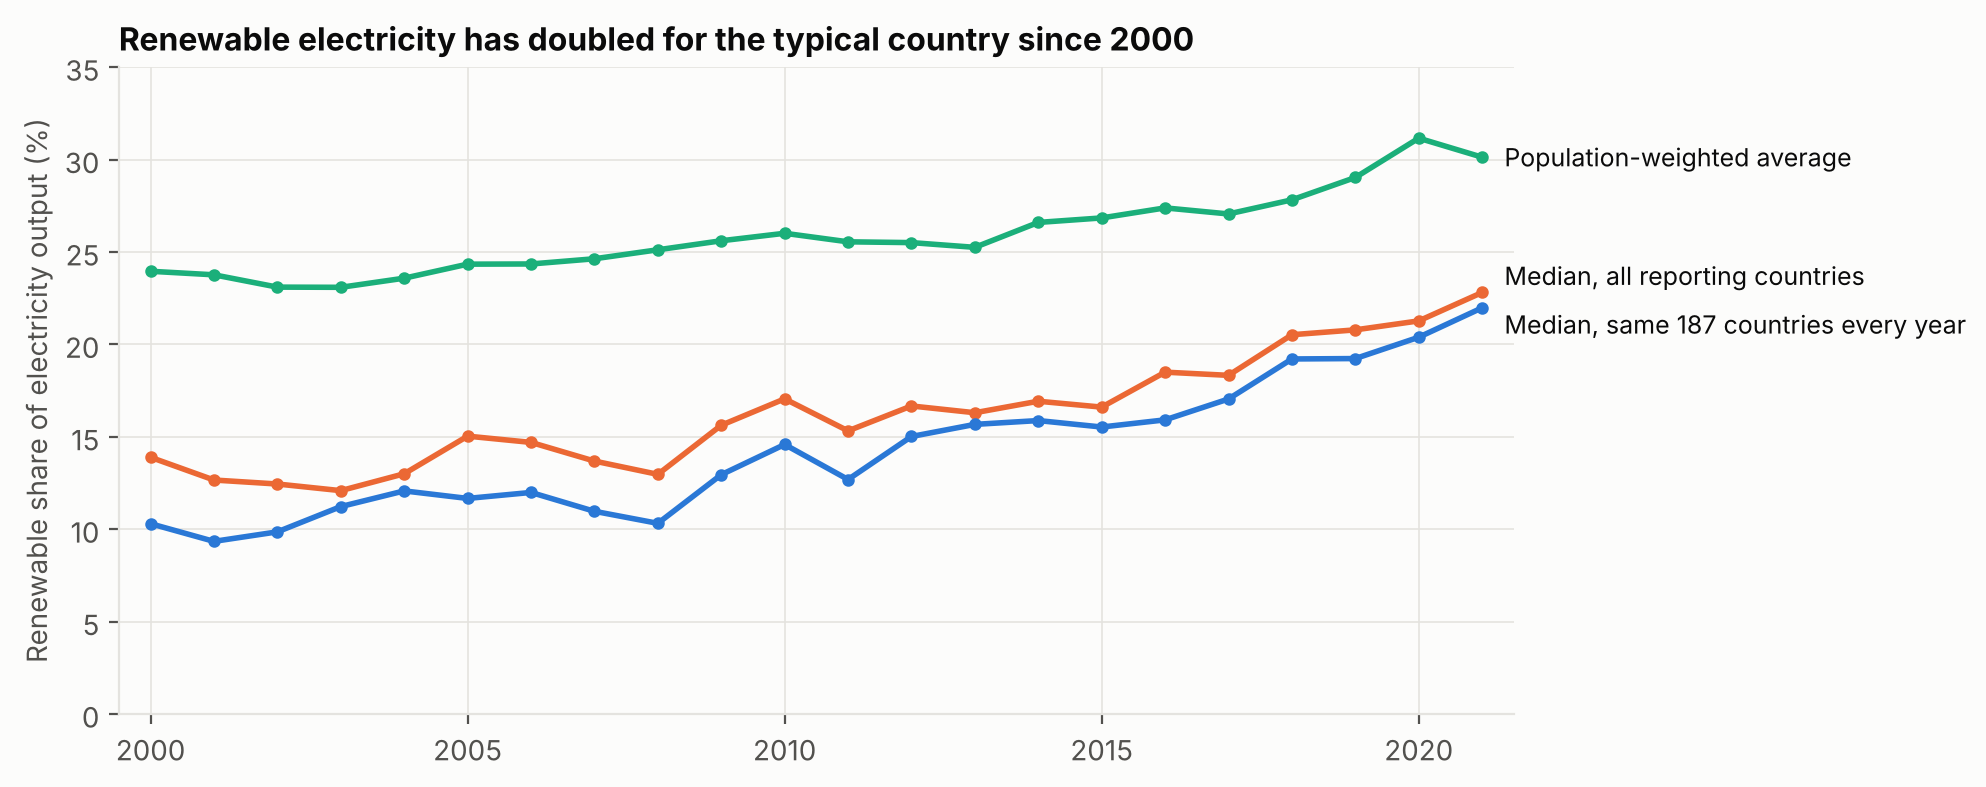
\includegraphics[width=0.92\textwidth]{figures/fig1_trend.png}
\caption{Renewable share of electricity, 2000--2021, measured three ways.}\label{fig:trend}
\end{figure}

\subsection{Q2: Income tells two different stories}

\begin{table}[H]
\centering\small
\caption{Median renewable shares by GDP per capita quartile, 2021.}\label{tab:quartiles}
\begin{tabular}{@{}lrrr@{}}
\toprule
\textbf{Quartile} & \textbf{Median GDP per capita} & \textbf{Electricity} & \textbf{All final energy} \\
\midrule
Q1 (poorest) & \$1,201 & 44\% & 65\% \\
Q2 & \$4,287 & 24\% & 19\% \\
Q3 & \$12,748 & 19\% & 13\% \\
Q4 (richest) & \$43,725 & 23\% & 12\% \\
\bottomrule
\end{tabular}
\end{table}

For all final energy, the renewable share falls steeply with income (Table~\ref{tab:quartiles}): Spearman $\rho = -0.56$ for both the World Bank series ($n=196$) and the UN SDG 7.2.1 series ($n=197$), $p<0.001$. In the poorest countries this mostly reflects traditional biomass for cooking. For electricity the association is weak ($\rho = -0.17$, $p = 0.019$, $n = 197$): rich countries range from almost no renewable electricity to almost all (Figure~\ref{fig:scatter}). ``Renewable share'' is therefore not a single measure of a clean-energy transition. The final-energy indicator partly tracks poverty and the electricity indicator partly tracks geography.

\begin{figure}[H]
\centering
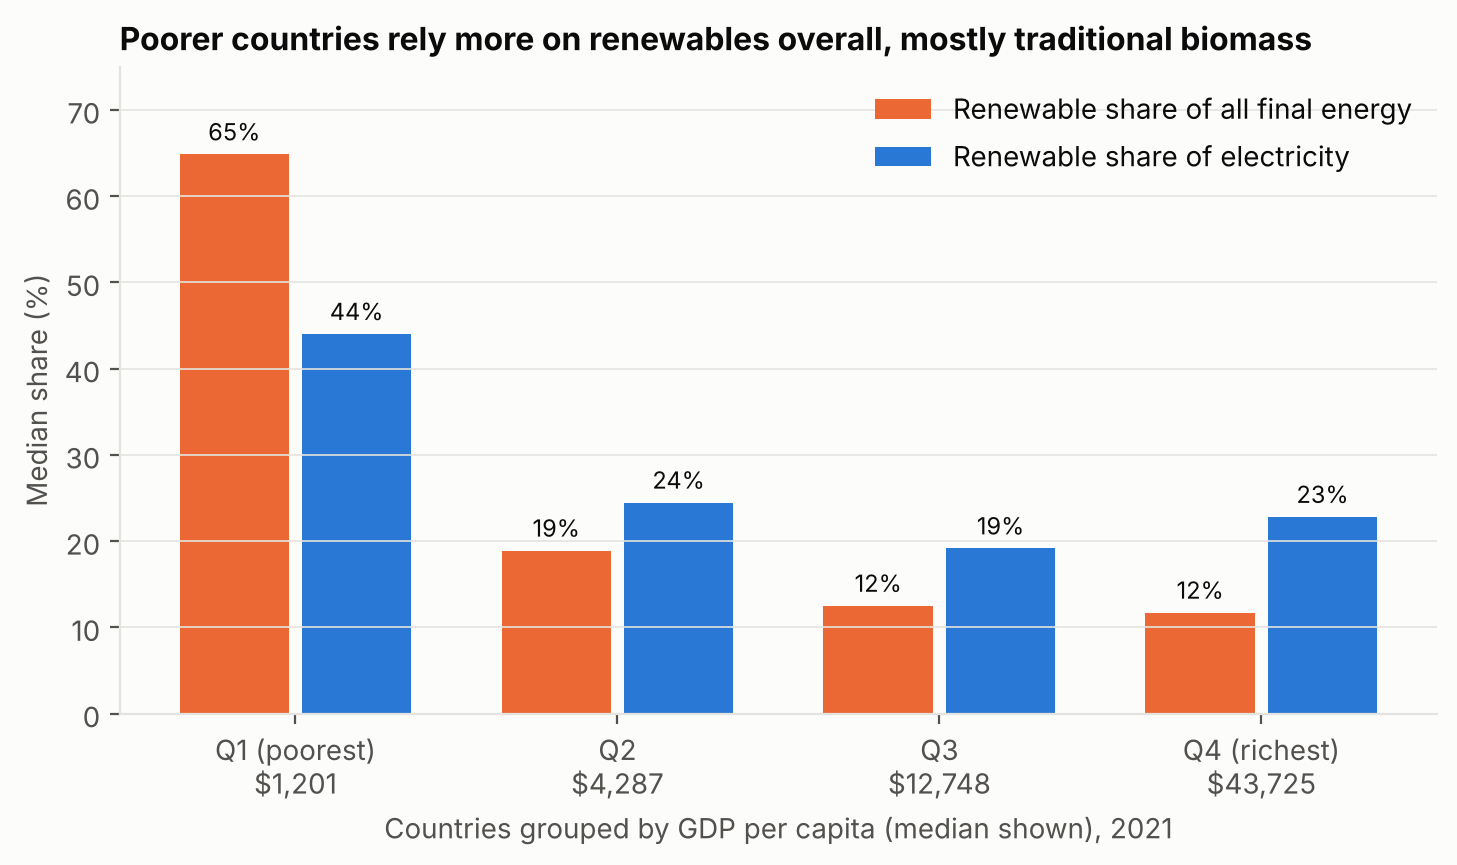
\includegraphics[width=0.82\textwidth]{figures/fig2_income_gradient.png}\\[4pt]
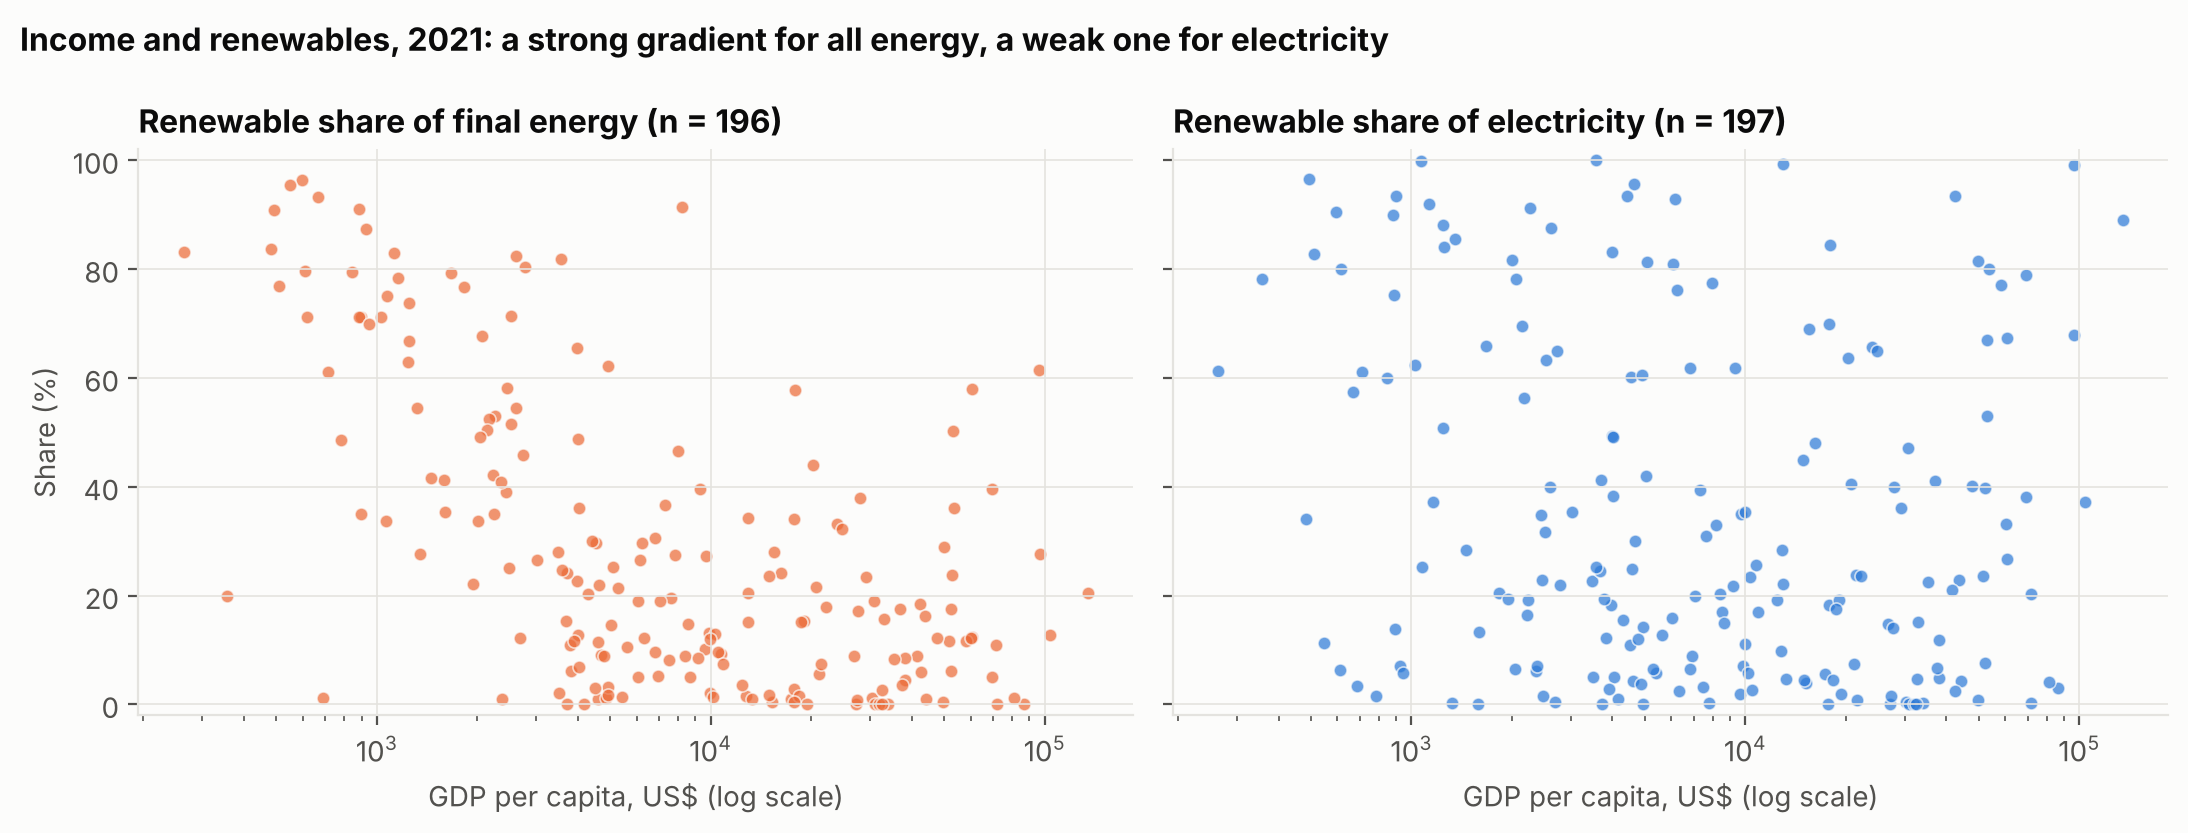
\includegraphics[width=\textwidth]{figures/fig3_gdp_scatter.png}
\caption{Top: median renewable shares by income quartile. Bottom: every country in 2021, GDP per capita on a log scale.}\label{fig:scatter}
\end{figure}

\subsection{Q3: Most countries moved up, and low-share countries are catching up}

Among the 151 countries with at least one million people, 74\% increased their renewable share of electricity between 2011 and 2021; the median change was $+4.6$\pp. The largest increases were in Cambodia ($+49.8$\pp, new hydropower), Denmark ($+38.7$, wind), Liberia ($+35.9$), Nicaragua ($+35.5$) and Djibouti ($+35.4$). The largest decreases were in Ghana ($-32.6$), the Republic of Congo ($-31.9$), Burundi ($-30.5$), Myanmar ($-22.1$) and Malawi ($-18.7$), all hydro-dependent systems. The usual explanations are demand growth met with new fossil generation, or droughts that cut hydro output (Figure~\ref{fig:changes}).

\begin{figure}[H]
\centering
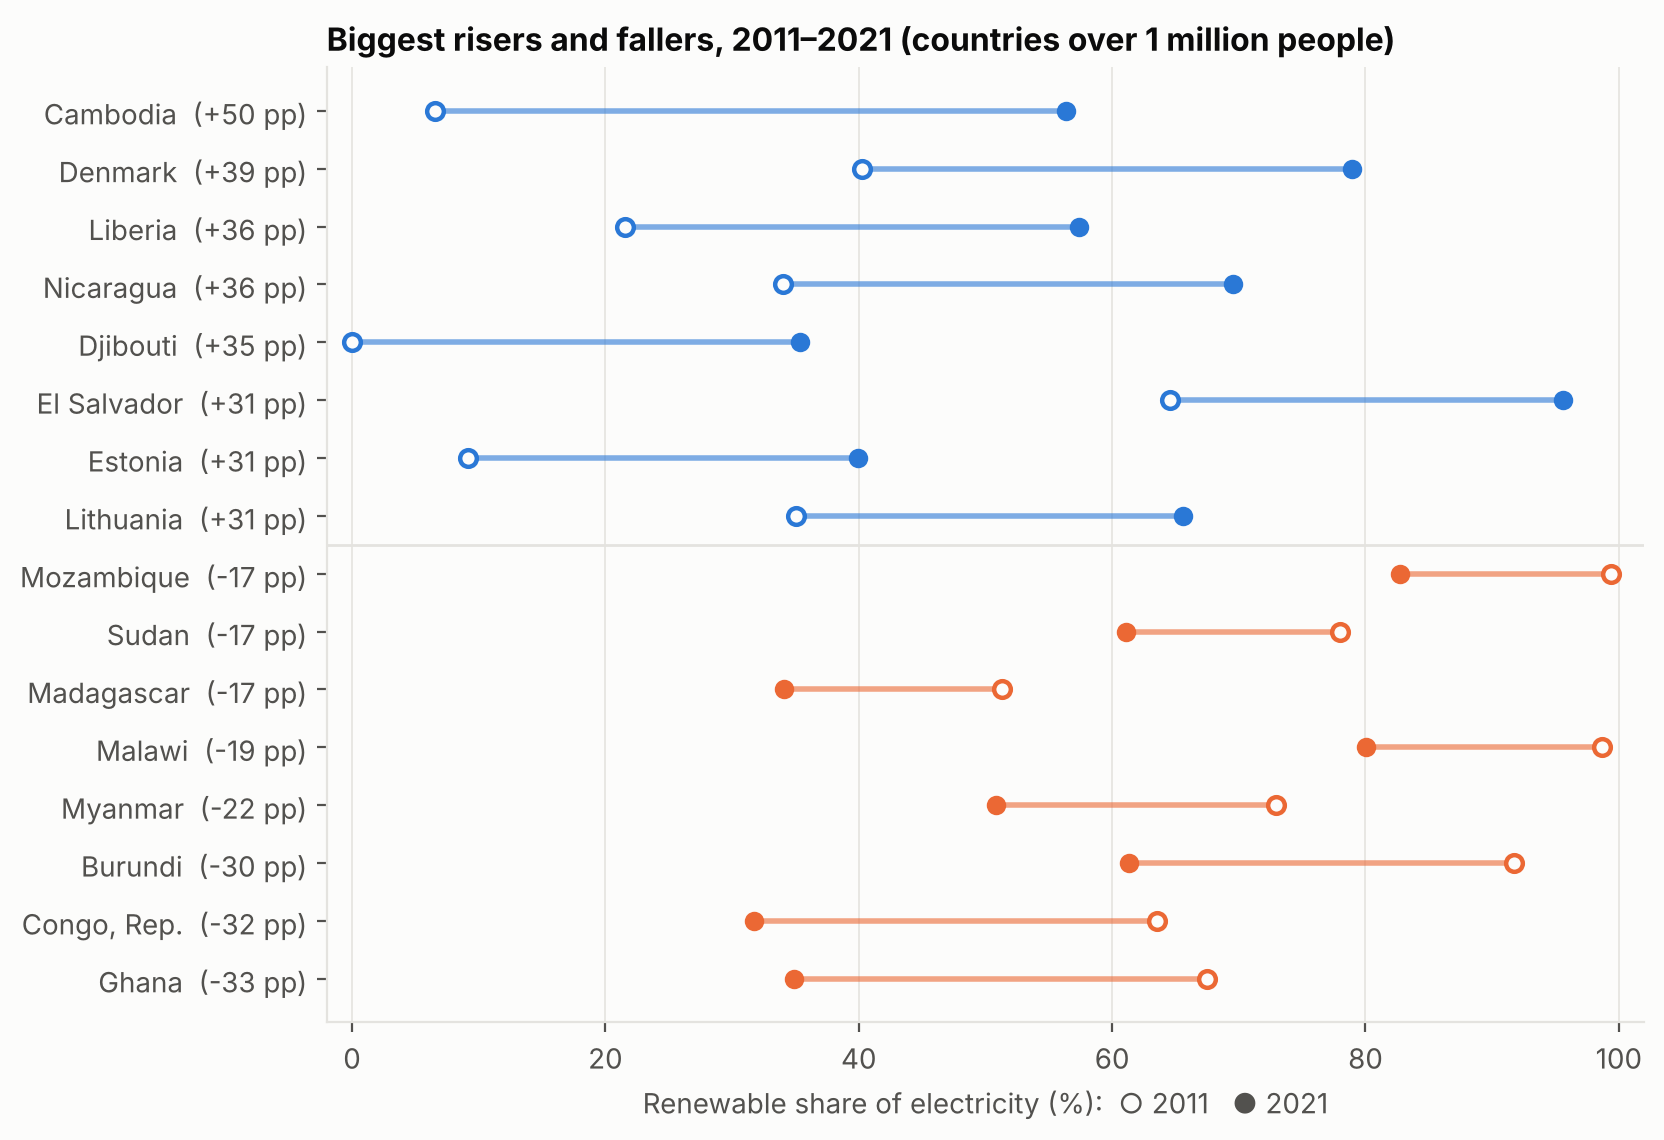
\includegraphics[width=0.8\textwidth]{figures/fig4_risers_fallers.png}
\caption{The eight largest increases and decreases, 2011--2021 (countries over one million people).}\label{fig:changes}
\end{figure}

Table~\ref{tab:models} summarises the regression models. Every coefficient, including those for the control variables, is listed in the repository's results files.

\begin{table}[H]
\centering\small
\caption{Regression results. HC3 robust standard errors, except Model 3 (clustered by country).}\label{tab:models}
\begin{tabularx}{\textwidth}{@{}Xlrcrrr@{}}
\toprule
\textbf{Model and outcome} & \textbf{Term} & \textbf{Estimate} & \textbf{95\% CI} & \textbf{$p$} & \textbf{$n$} & \textbf{$R^2$} \\
\midrule
\multirow{3}{=}{1. Electricity share, 2021} & log GDP per capita & $-6.61$ & $[-10.82,\ -2.40]$ & 0.002 & 197 & 0.15 \\
 & log population & $2.45$ & $[0.38,\ 4.51]$ & 0.020 & & \\
 & Europe (vs Africa) & $22.48$ & $[5.63,\ 39.33]$ & 0.009 & & \\
\addlinespace
\multirow{2}{=}{1. Final-energy share, 2021} & log GDP per capita & $-9.18$ & $[-12.06,\ -6.30]$ & $<$0.001 & 205 & 0.49 \\
 & Asia (vs Africa) & $-26.43$ & $[-37.54,\ -15.31]$ & $<$0.001 & & \\
\addlinespace
\multirow{4}{=}{2. Change in electricity share, 2011--2021} & Starting share, 2011 & $-0.110$ & $[-0.171,\ -0.049]$ & $<$0.001 & 149 & 0.25 \\
 & log GDP per capita & $-0.11$ & $[-1.80,\ 1.58]$ & 0.896 & & \\
 & Europe (vs Africa) & $12.93$ & $[6.48,\ 19.38]$ & $<$0.001 & & \\
 & America (vs Africa) & $8.50$ & $[1.49,\ 15.51]$ & 0.018 & & \\
\addlinespace
3. Electricity share, 2000--2021, country and year fixed effects & log GDP per capita & $-2.46$ & $[-5.51,\ 0.59]$ & 0.113 & 4,312 & \\
\bottomrule
\end{tabularx}
\end{table}

\begin{itemize}
  \item \textbf{Convergence.} Each 10 points of starting share in 2011 means about 1.1 points less growth by 2021 ($\hat\beta = -0.110$, $p<0.001$). Once the starting share is known, income adds nothing ($p = 0.90$). European countries gained about 13 points more than comparable African countries. Part of this is regression to the mean and the 100\% ceiling (Section~\ref{sec:models}), but the pattern holds across the whole range (Figure~\ref{fig:convergence}).
  \item \textbf{Income across countries.} With continent and population held fixed, richer countries have lower renewable shares of electricity: $-6.61$ points per log unit, or about $-15$ points for a tenfold difference in income. The model explains only 15\% of the variation, compared with 49\% for final energy. Clean electricity depends mainly on factors not in the data, such as hydro resources and policy.
  \item \textbf{Income within countries.} In the fixed-effects model the estimate is negative but not statistically significant ($p = 0.11$). The cross-country income pattern should not be read as a path that individual countries follow as they grow richer.
\end{itemize}

\begin{figure}[H]
\centering
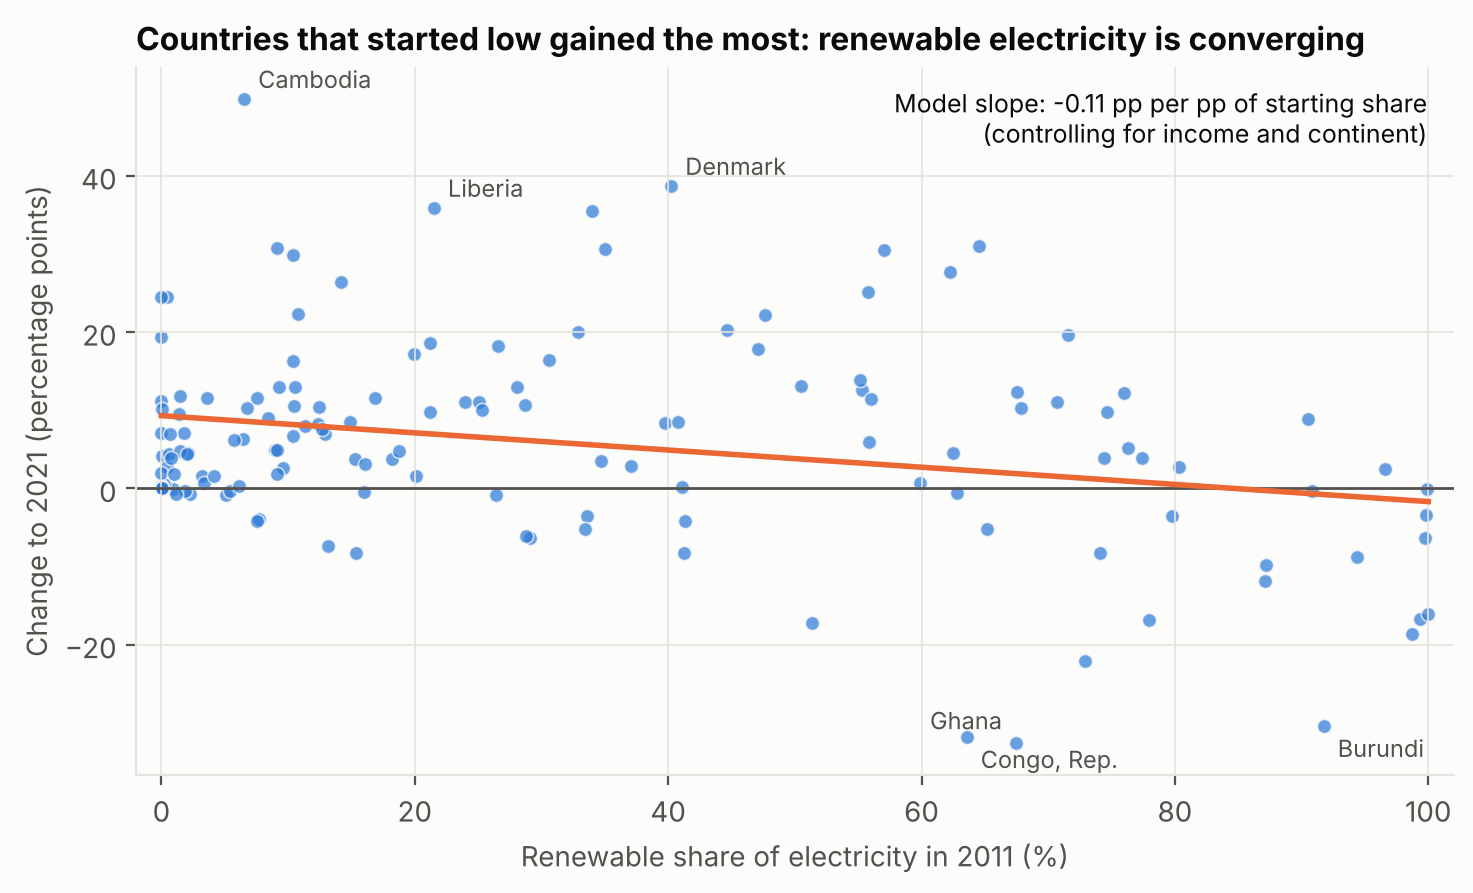
\includegraphics[width=0.82\textwidth]{figures/fig5_convergence.png}
\caption{Starting share in 2011 against change to 2021. The line has the slope from Model 2.}\label{fig:convergence}
\end{figure}

\subsection{Q4: The electricity mix up to 2024}

Ember's data extend the picture to 2024 and separate the sources (Table~\ref{tab:mix}). Worldwide, renewables rose from 18.7\% of electricity in 2000 to 31.9\% in 2024, and wind and solar together from 0.2\% to 15.0\%. Total generation roughly doubled (15,279 to 30,930\,TWh), so fossil generation also grew: coal added 4,730\,TWh and gas 4,137\,TWh between 2000 and 2024, while wind and solar added 4,620\,TWh together. Coal remained the largest single source in 2024 (34.1\%).

\begin{table}[H]
\centering\small
\caption{Electricity mix in selected countries, 2000 and 2024 (share of total generation).}\label{tab:mix}
\begin{tabular}{@{}lrrrrrr@{}}
\toprule
 & \multicolumn{2}{c}{\textbf{Renewables}} & \multicolumn{2}{c}{\textbf{Wind and solar}} & \multicolumn{2}{c}{\textbf{Coal}} \\
\cmidrule(lr){2-3}\cmidrule(lr){4-5}\cmidrule(l){6-7}
\textbf{Country} & 2000 & 2024 & 2000 & 2024 & 2000 & 2024 \\
\midrule
World & 18.7\% & 31.9\% & 0.2\% & 15.0\% & 38.0\% & 34.1\% \\
China & 16.6\% & 33.7\% & 0.0\% & 18.2\% & 78.2\% & 57.8\% \\
United States & 9.2\% & 24.1\% & 0.2\% & 17.2\% & 51.7\% & 14.9\% \\
India & 14.0\% & 19.8\% & 0.3\% & 11.0\% & 68.3\% & 74.5\% \\
Germany & 6.2\% & 58.6\% & 1.6\% & 43.5\% & 52.1\% & 21.4\% \\
United Kingdom & 2.6\% & 50.6\% & 0.2\% & 34.5\% & 31.8\% & 0.7\% \\
Denmark & 15.5\% & 89.2\% & 11.8\% & 69.0\% & 46.5\% & 5.0\% \\
Brazil & 89.5\% & 87.3\% & 0.0\% & 24.1\% & 3.1\% & 2.2\% \\
South Africa & 0.8\% & 12.5\% & 0.0\% & 11.9\% & 93.1\% & 83.6\% \\
\bottomrule
\end{tabular}
\end{table}

Three patterns stand out. First, countries such as the United Kingdom, Germany and Denmark show a genuine fuel switch: coal nearly disappears and wind and solar take its place. Second, in fast-growing systems such as India, wind and solar grow quickly but demand grows faster, so coal's share can still rise. Third, hydro-based systems such as Brazil keep a stable renewable share while wind and solar replace part of the hydro, which the World Bank share series cannot show.

% ================================================================= 6
\section{The interactive dashboard}\label{sec:dashboard}

The dashboard \citep{dashboard} is a single self-contained web page built by the same pipeline and published with GitHub Pages. It has three sections:

\begin{enumerate}
  \item \textbf{Explore a country} (Figure~\ref{fig:dash-explorer}): pick the world or any of 214 countries to see summary figures, a stacked area chart of generation by source from 2000 to 2024 (in TWh or as a share), and a Sankey diagram of the electricity flow for any year chosen with a slider. A sentence summarising the change is generated for each country.
  \item \textbf{Renewable electricity around the world} (Figure~\ref{fig:dash-map}): a world map shaded by renewable share, with a year slider from 2000 to 2021.
  \item \textbf{Are richer countries more renewable?}: the income scatter plot, with a switch between electricity and all energy use.
\end{enumerate}

\begin{why}[Design choices]
The page uses one fixed light theme so that it looks the same in every browser and operating-system setting and when printed. Each chart has a plain-language heading, a line on how to read it and a takeaway sentence, so that a reader without a background in energy can follow it. Countries with no data are shown in grey rather than in the lightest colour, so that missing data are not mistaken for 0\%.
\end{why}

\begin{figure}[H]
\centering
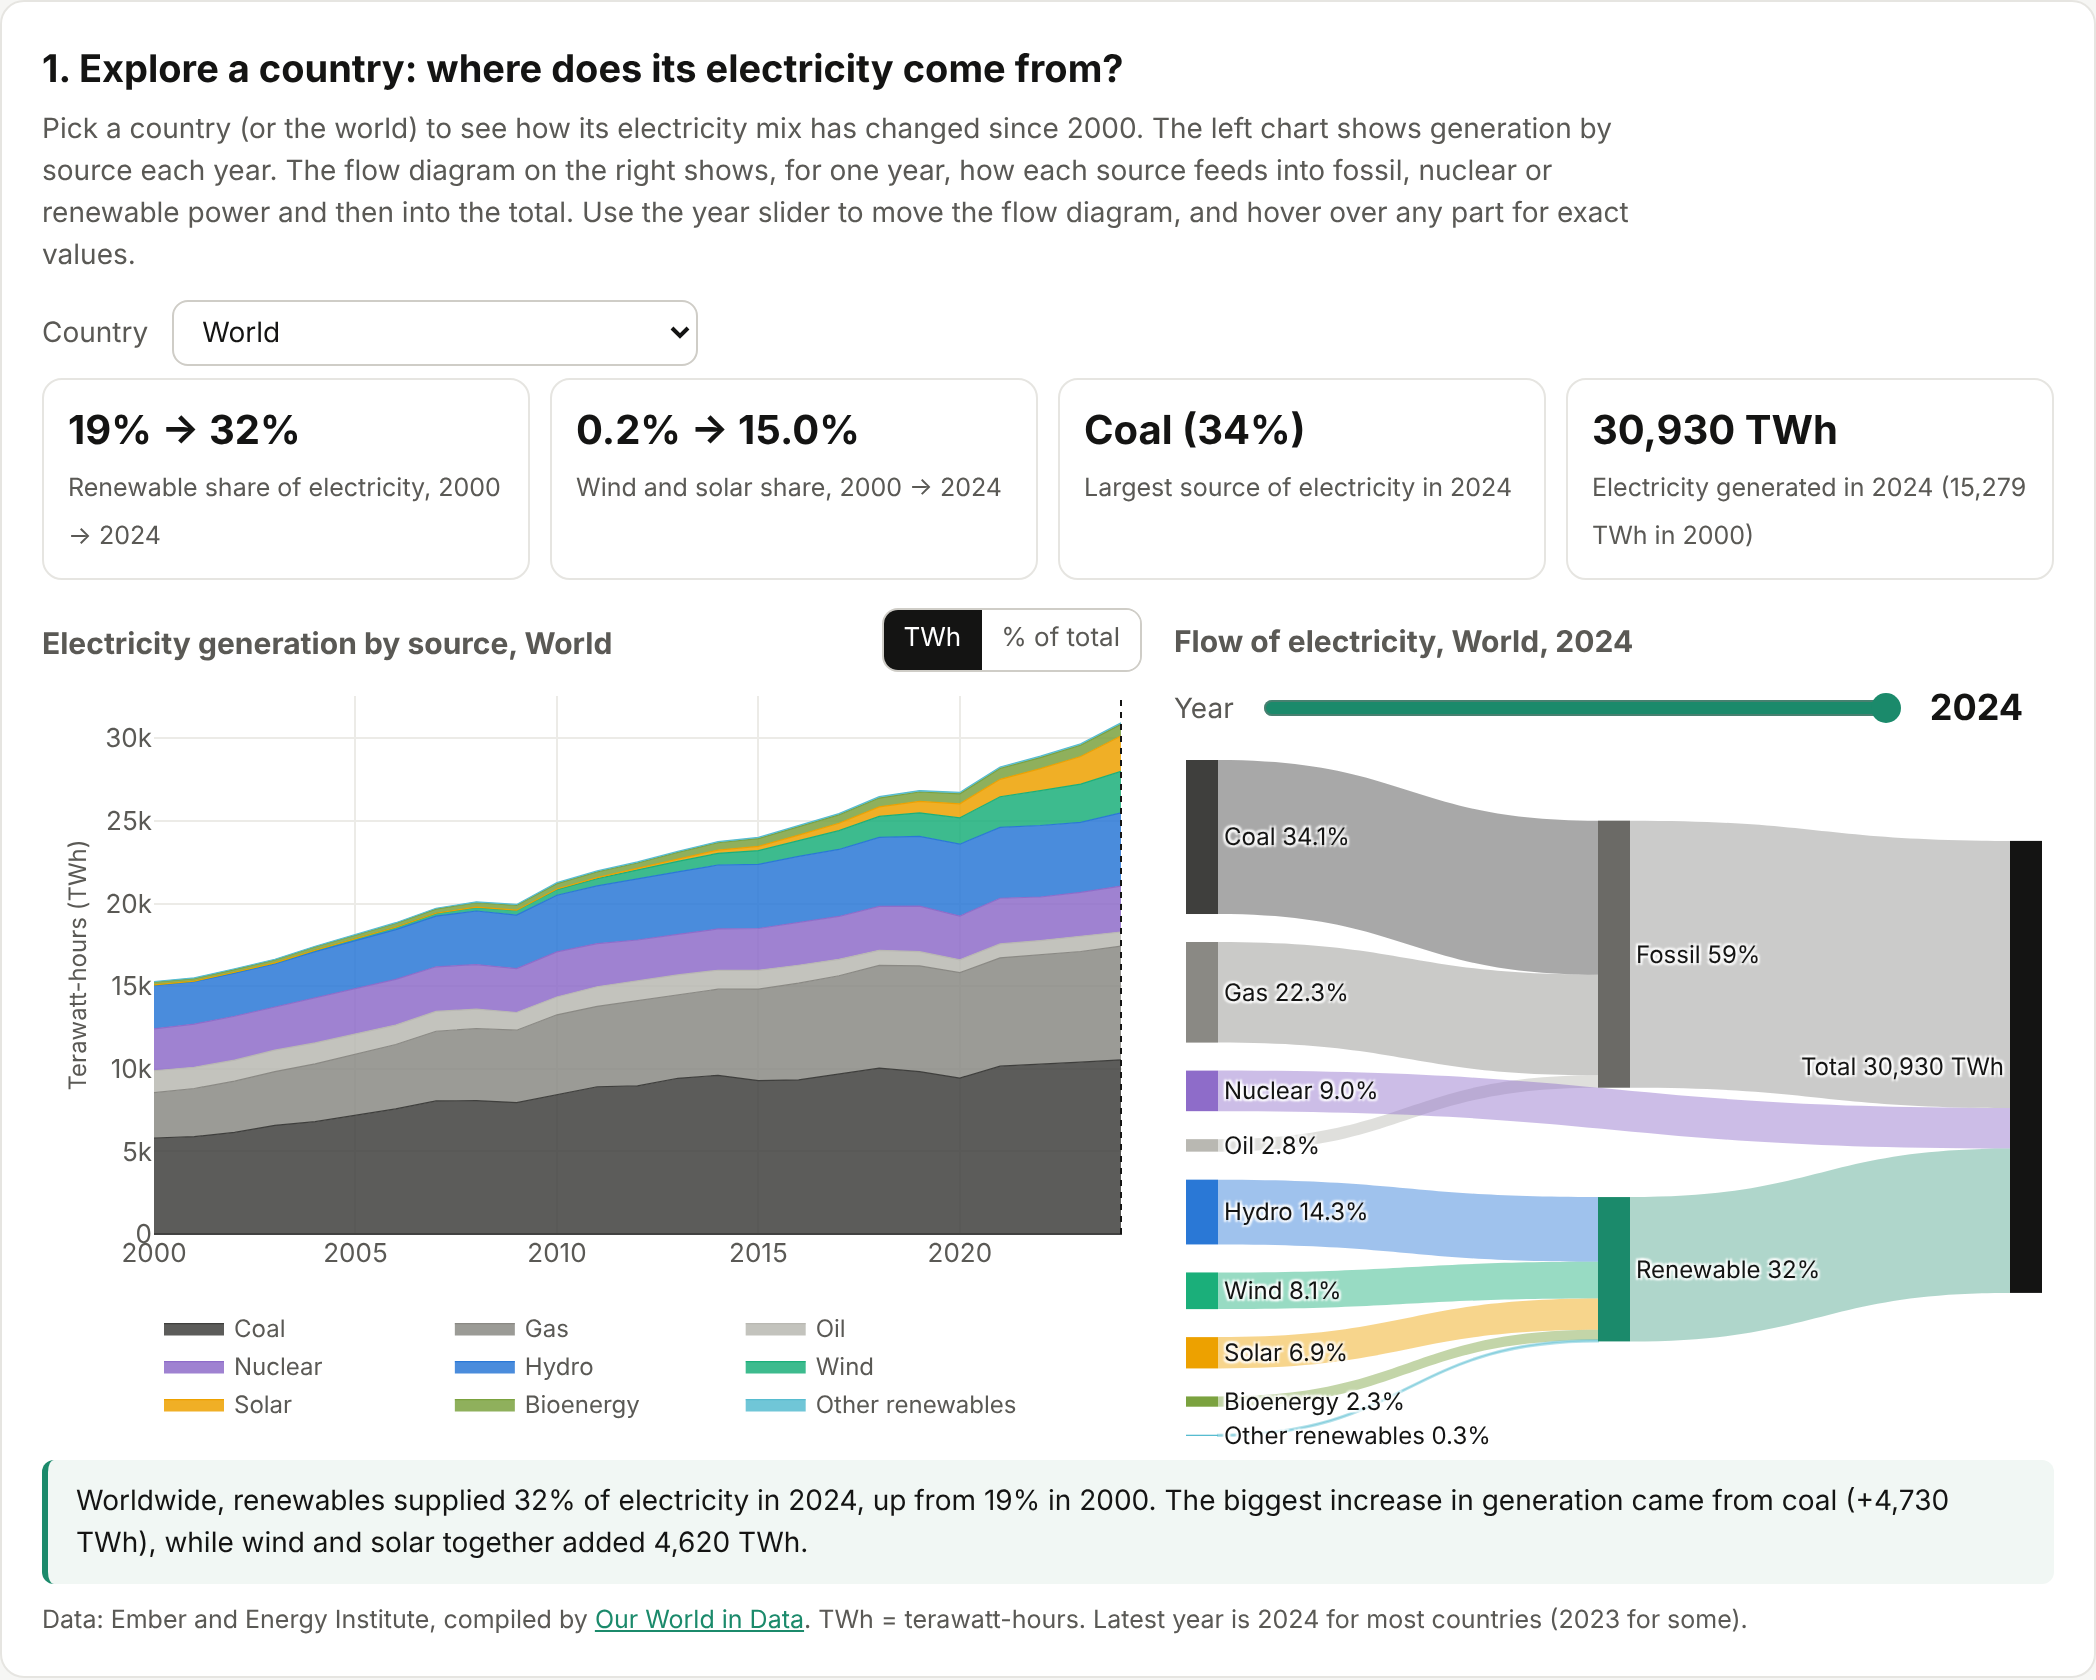
\includegraphics[width=\textwidth]{figures/dashboard_explorer.png}
\caption{Dashboard, section 1: the country explorer, showing the world in 2024.}\label{fig:dash-explorer}
\end{figure}

\begin{figure}[H]
\centering
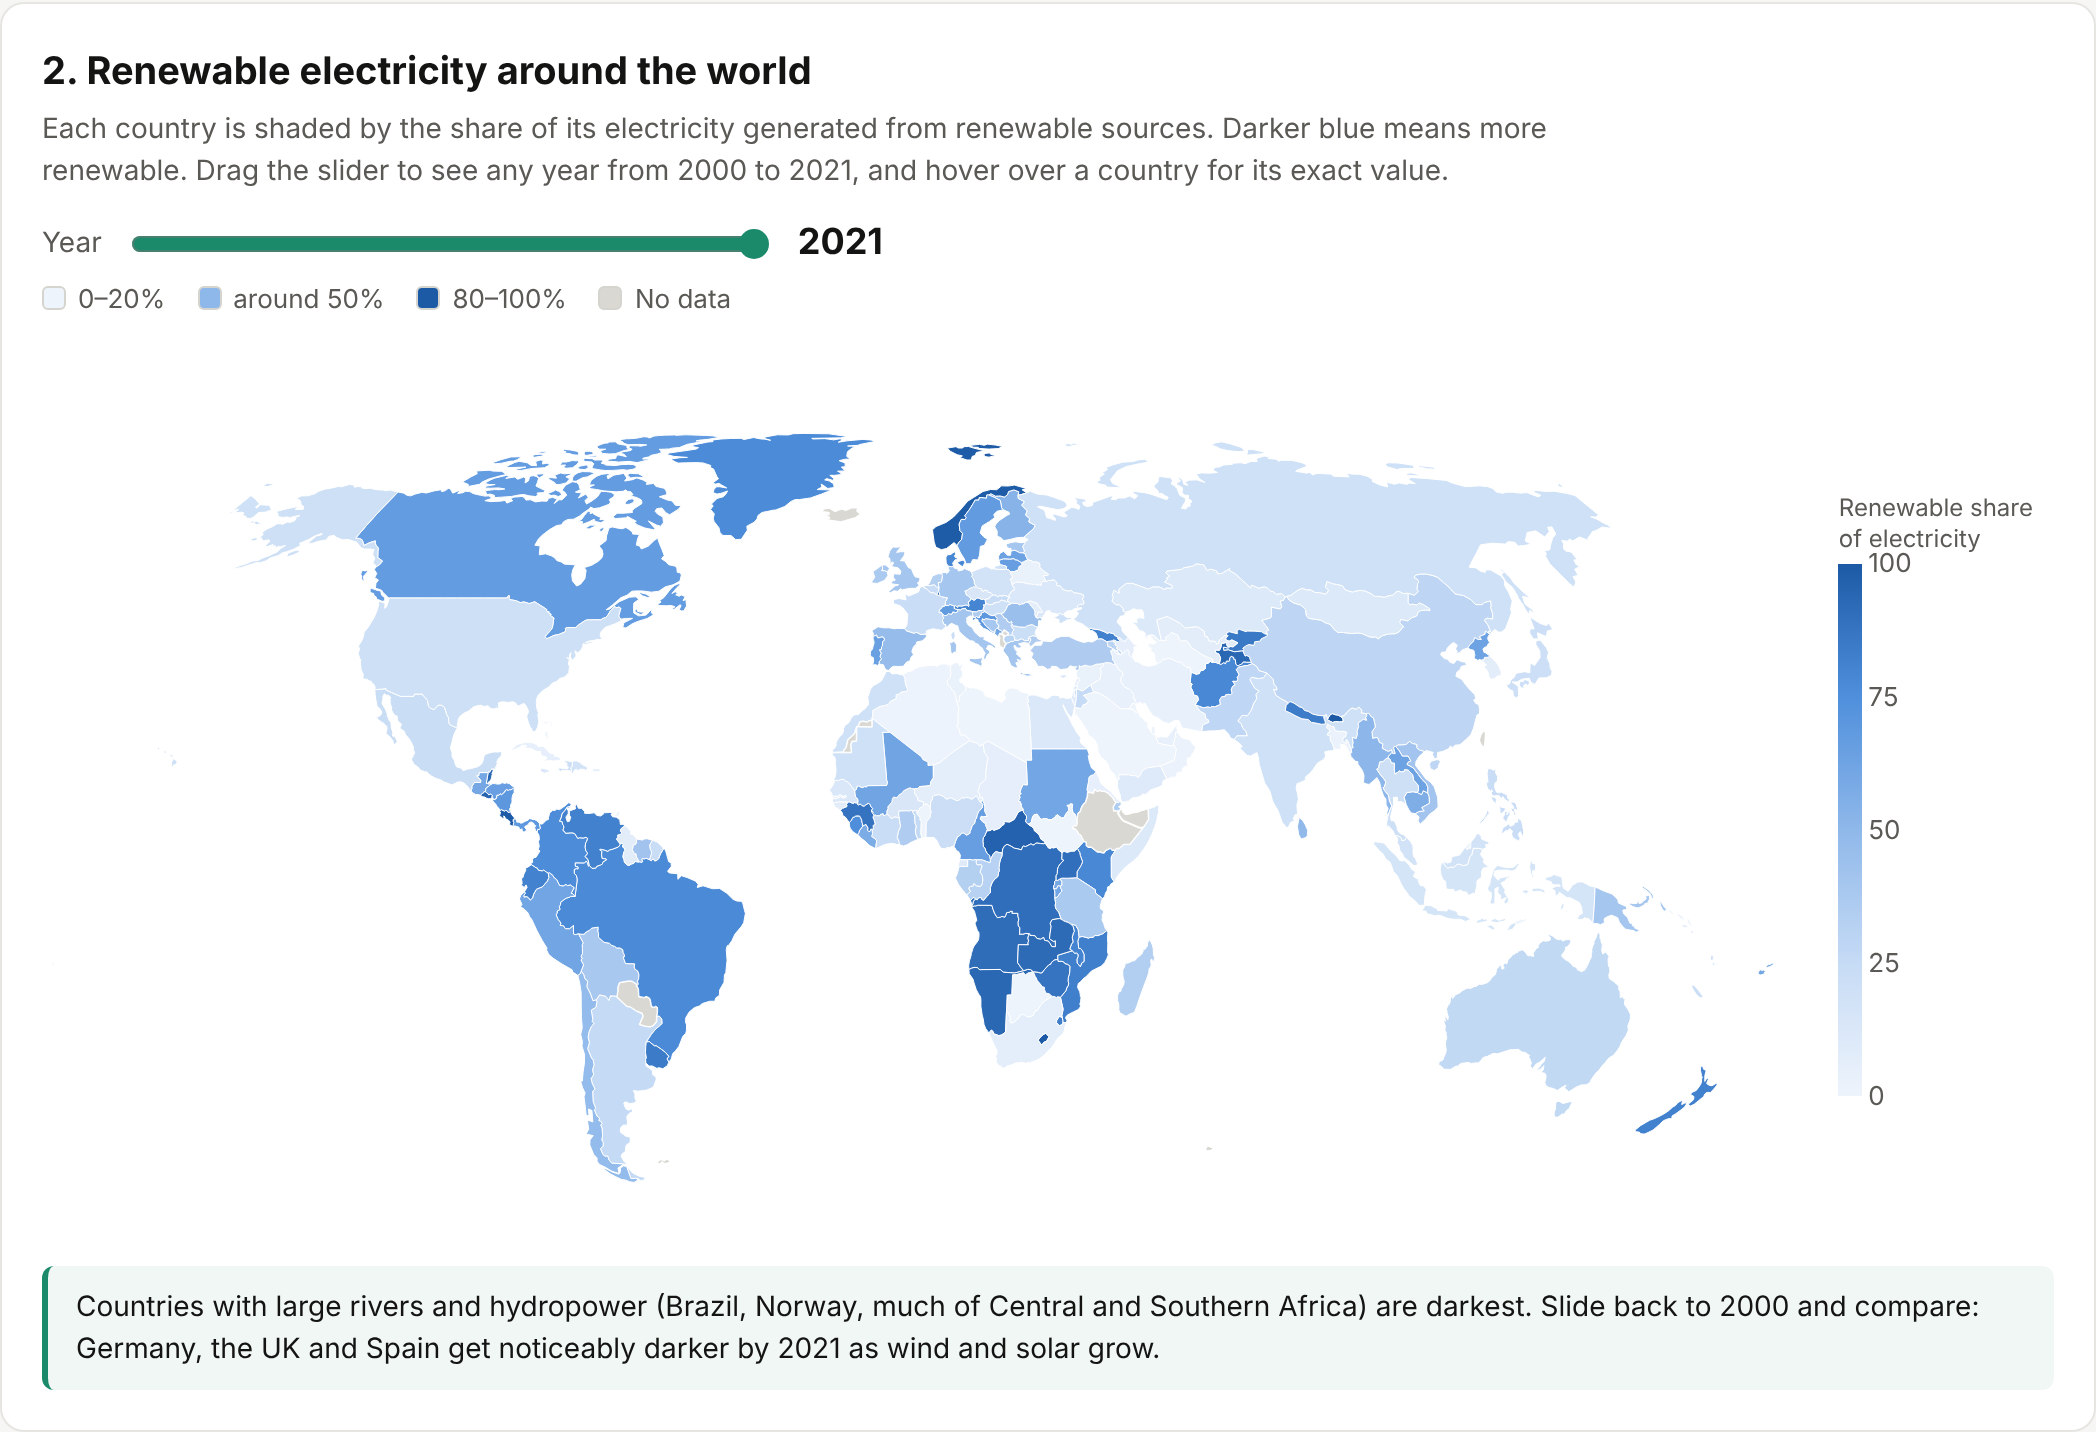
\includegraphics[width=0.9\textwidth]{figures/dashboard_map.png}
\caption{Dashboard, section 2: renewable share of electricity by country.}\label{fig:dash-map}
\end{figure}

% ================================================================= 7
\section{Reproducibility and quality checks}\label{sec:repro}

\begin{itemize}
  \item \textbf{Raw data stored unchanged.} Every input is stored in \code{data/raw/} exactly as downloaded (gzipped), so the analysis does not depend on an API returning the same data later.
  \item \textbf{One command rebuilds everything}: clean tables, results, figures and the dashboard.
  \item \textbf{Automated tests} (11 with pytest) check that only countries are kept, that every percentage lies between 0 and 100, the UN series and its coverage, the balanced panel, the headline numbers, the quartiles, the small-country filter, continent coverage, the sign and significance of the convergence coefficient, and that electricity sources add up to the total.
  \item \textbf{Continuous integration.} On every change, GitHub Actions lints the code, runs the tests and rebuilds all outputs from the raw data. The build fails if any committed result changes.
  \item \textbf{Determinism.} Library versions are fixed in \code{requirements-lock.txt}; summary statistics are rounded to six significant figures so they do not change in the last digit between environments; and every sort uses a unique key. The last point came from a real failure: sorting on a key with ties gave a different order on GitHub's servers than locally, because NumPy's default sort can use processor-specific instructions.
\end{itemize}

% ================================================================= 8
\section{Limitations}\label{sec:limitations}

\begin{itemize}
  \item \textbf{No causal claims.} All results are associations. Income, geography, resource endowments and policy are intertwined, and nothing here identifies the causal effect of any of them.
  \item \textbf{Missing explanatory variables.} The models have no measures of hydro, wind or solar resources, energy prices or policy (feed-in tariffs, auctions, carbon pricing). This likely explains most of the unexplained variation in renewable electricity.
  \item \textbf{Income measure.} GDP per capita is in current US dollars. Constant-price, purchasing-power-parity GDP would be better for comparing countries and years.
  \item \textbf{Convergence estimate.} Regression to the mean and the 100\% ceiling push the convergence coefficient downward; it is an upper bound on the speed of catching up. A robustness check using a multi-year average starting share is left for future work.
  \item \textbf{Equal weighting.} Country medians give every country equal weight. The population-weighted mean is not a generation-weighted global share; the world figures from Ember are the right measure of the global mix.
  \item \textbf{Data periods differ.} The World Bank renewable electricity series ends in 2021, while Ember runs to 2024 (2023 for some countries). UN SDG 7.2.1 has only 84 of 225 values for 2024, so 2023 is the latest comparable year.
  \item \textbf{Overlapping sources.} The World Bank and UN final-energy series draw on overlapping underlying data and are not independent confirmations of each other.
\end{itemize}

% ================================================================= 9
\section{Conclusions and next steps}\label{sec:conclusion}

Renewable electricity grew in most countries between 2000 and 2024, and the typical country's share doubled. How the trend is measured changes the headline, and a renewable share means different things for electricity and for all energy use: in the poorest countries a high share reflects reliance on traditional biomass. Countries that started low are catching up, and income explains little of who has clean electricity, either across countries or within a country over time. The electricity data up to 2024 show that the transition is real but uneven: some countries are replacing coal with wind and solar, while in others clean generation is growing but not yet faster than demand.

The natural next step is to model wind and solar adoption directly with Ember's source-level data, adding resource potential, electricity demand growth and policy variables, and replacing current-dollar GDP with constant PPP GDP. That would move the project from describing patterns to testing explanations of why some countries move faster than others.

% ================================================================= references
\clearpage
\bibliographystyle{plainnat}
\bibliography{references}

% ================================================================= appendices
\clearpage
\appendix
\section{Repository structure and how to reproduce}\label{app:repo}

\begin{tabularx}{\textwidth}{@{}lX@{}}
\toprule
\textbf{Path} & \textbf{Contents} \\
\midrule
\code{src/energy\_transition/} & \code{build.py} (raw to clean), \code{analysis.py}, \code{models.py}, \code{figures.py}, \code{dashboard.py} \\
\code{data/raw/} & World Bank and UN API responses, Our World in Data energy file (gzipped, unchanged) \\
\code{data/clean/} & Country--year tables used by the analysis \\
\code{results/} & \code{summary.json} and one CSV per table, including \code{model\_coefficients.csv} \\
\code{figures/} & Static figures \\
\code{docs/} & Dashboard (\code{index.html}), research note, data dictionary, this report \\
\code{tests/} & Data and results checks \\
\bottomrule
\end{tabularx}

\medskip
\noindent To reproduce every result:
\begin{verbatim}
git clone https://github.com/sahiljangra12/energy-transition-analysis
cd energy-transition-analysis
pip install -e ".[dev]" -c requirements-lock.txt
python -m energy_transition       # rebuild data, results, figures, dashboard
pytest                               # run the checks
\end{verbatim}

\noindent To rebuild this report, open \code{docs/technical-report/} in Overleaf (upload the folder as a zip) or run \code{make} in that folder.

\section{Software versions}\label{app:versions}

\begin{tabular}{@{}ll@{\hspace{2cm}}ll@{}}
\toprule
\textbf{Package} & \textbf{Version} & \textbf{Package} & \textbf{Version} \\
\midrule
Python & 3.13 & statsmodels & 0.15.0 \\
pandas & 3.0.6 & matplotlib & 3.11.2 \\
NumPy & 2.5.4 & pycountry & 26.2.16 \\
SciPy & 1.18.1 & country\_converter & 1.3.2 \\
patsy & 1.0.3 & Plotly.js & 2.35.2 \\
pytest & 9.1.1 & Ruff & 0.17.0 \\
\bottomrule
\end{tabular}

\end{document}
